\section{Part~V: Unified Failure Phase Space}\label{sec:part5}

The previous sections rigorously characterized PINN failure by isolating individual hyperparameters at fixed, discrete parameter values. While highly informative for diagnosing specific pathologies, this 1D approach obscures the complex interdependencies between the network's spatial resolution, its internal capacity, and the underlying stiffness of the governing equations. This section maps how failure modes transition dynamically as two critical parameters are varied simultaneously. By treating the convergence status as a physical state, we produce expansive 2D phase diagrams mathematically analogous to thermodynamic phase boundaries. Critically, the empirical data reveals that these boundaries are not smooth, continuously differentiable curves amenable to parametric fitting—they are steep convergence cliffs where the network transitions instantaneously from trivially solvable to structurally impossible.

\subsection{Grid Design and Classification Protocol}\label{sec:exp25}\label{sec:phaseintro}

To systematically map the failure boundaries across diverse regimes, we defined three independent parameter grids: Grid A ($\betaAdv$ versus collocation density $\Ncol$), Grid B (Burgers viscosity $\nuBurg$ versus $\Ncol$), and Grid C ($\betaAdv$ versus architecture width). Each configuration was trained for a budget of $40{,}000$ epochs—matching the paper's main-text default (Table~\ref{tab:app_budgets})—with early stopping triggered when a model sustained $\Ltwo < 0.02$ across three consecutive evaluation checkpoints. This design ensures that easy configurations (e.g., $\betaAdv=1$) exit in a few thousand epochs, while genuinely hard configurations near or at the failure boundary receive the full training budget.

Upon completion of the training budget, each model was programmatically evaluated and assigned a rigid regime classification using the multi-metric threshold criteria established in Section~\ref{sec:methods}. Configurations achieving a relative $\Ltwo < 0.1$ were designated as SUCCESS. Failing models were further stratified into specific structural failure modes---Spectral Bias ($\Ltwo > 0.5$, gradient ratio below threshold), Gradient Pathology (gradient ratio $> 20$), or Unclassified (ambiguous intermediate band $\Ltwo \in (0.1, 0.5]$ with no dominant diagnostic signal)---based on their terminal loss ratios and gradient diagnostic metrics. A \emph{triple-point regime} — by analogy to thermodynamic phase diagrams, a locus where three distinct failure regimes converge simultaneously — might be expected near the intersection of spectral bias, gradient pathology, and success boundaries. However, none of the three parameter grids surveyed here resolves such a region: Grid~A shows a sharp spectral-bias boundary but no co-occurrence of all three regimes in a single cell or adjacent cell cluster; Grid~B exhibits only a two-regime transition (success to gradient pathology); Grid~C is similarly two-regime. We report this \emph{absence} as an empirical finding: within the tested parameter ranges, the failure boundaries are sharp and non-intersecting rather than converging at a triple point. Whether a triple-point exists at finer grid resolution or at intermediate $\beta / \nu$ values remains an open question.

\subsection{Grid A: Advection Stiffness vs Collocation Density}

Grid A maps the baseline 1D advection problem across a severe stiffness domain spanning $\betaAdv \in [1, 50]$ against an interior point density domain spanning $\Ncol \in [100, 5000]$. The resulting empirical phase diagram reveals a strictly bounded convergence zone that does not narrow gradually—it terminates abruptly.

For $\betaAdv \le 5$, the PINN converges successfully across all tested collocation densities, including the minimum $\Ncol = 100$. For $\betaAdv = 10$, a single transition is observed: the network fails at $\Ncol = 100$ but succeeds for all $\Ncol \ge 250$. However, for $\betaAdv \ge 20$, \emph{every configuration fails unconditionally}—even at the maximum $\Ncol = 5{,}000$—with terminal $\Ltwo$ values in the range $0.79$--$0.95$. This constitutes an abrupt performance cliff: the transition from universal success to universal failure occurs between $\betaAdv = 10$ and $\betaAdv = 20$ with no intermediate recovery region. Massively scaling the collocation budget by $50\times$ (from $100$ to $5{,}000$) yields zero measurable recovery once the stiffness exceeds this critical threshold.

This discontinuity has a direct structural interpretation. At $\betaAdv \ge 20$, the characteristic spatial frequency of the exact solution $u(x,t) = \sin(x - \betaAdv t)$ exceeds the effective bandwidth of the Neural Tangent Kernel at initialization, as quantified in Exp.~3. Because the NTK bandwidth is an architectural constant that does not scale with collocation density, adding more training data cannot resolve a frequency that the kernel is structurally blind to. The failure is not one of insufficient sampling—it is one of representational impossibility.

The regime classification at the highest stiffness values ($\betaAdv = 50$) reveals gradient pathology (code 2) at low $\Ncol$ transitioning to spectral bias (code 1) at higher $\Ncol$, indicating that the two failure mechanisms partition the failure space rather than overlapping. This transition is consistent with the finding in Section~\ref{sec:phaseintro} that no triple-point regime was resolved across any tested grid; instead, the regime boundaries converge into a hard, right-angle cliff near $\betaAdv \approx 10$--$20$, where the phase diagram transitions from a uniformly green (success) region to a uniformly blue/orange (failure) region with no gradual mixing zone.

\begin{figure}[h!]
    \centering
    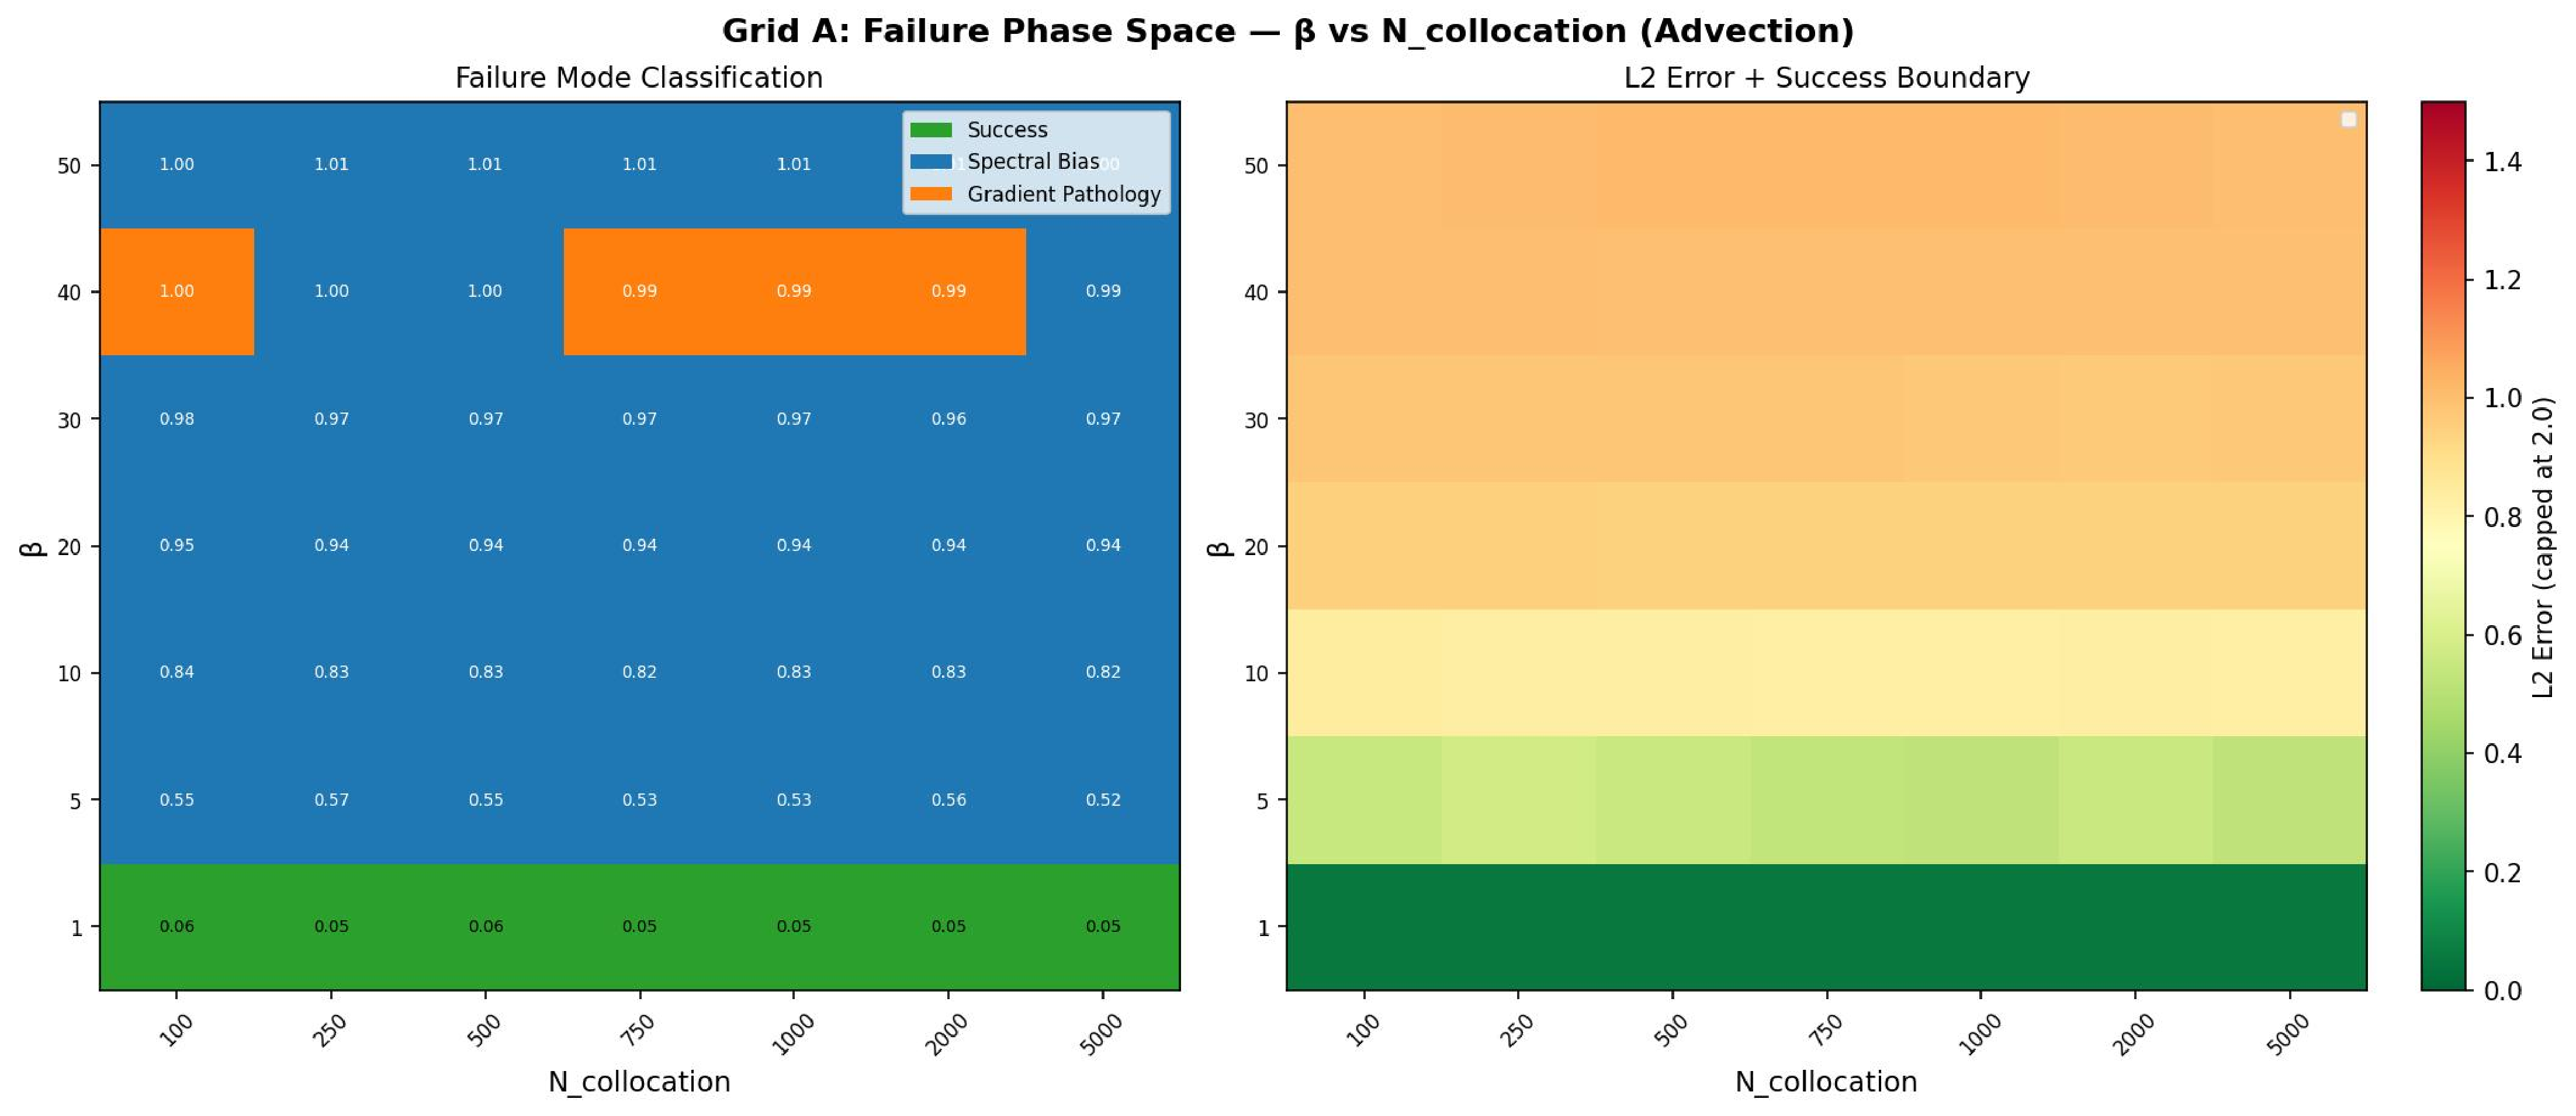
\includegraphics[width=\linewidth]{results/exp25/phase_map_beta_N.pdf}
    \caption{Phase map for Grid A ($\betaAdv$ vs $\Ncol$). A steep convergence cliff is visible between $\betaAdv = 10$ (universally successful for $\Ncol \ge 250$) and $\betaAdv = 20$ (universally failed across all $\Ncol$). No smooth boundary curve can be fitted to this transition because only a single transition point exists in the entire grid. The regime classification shifts from gradient pathology to spectral bias at the highest $\betaAdv$ rows.}
    \label{fig:exp25_gridA}
\end{figure}

\subsection{Grid B: Burgers Viscosity vs Collocation Density}

Grid B transitions the analytical focus to the highly non-linear Viscous Burgers equation, mapping the viscosity parameter across a physically stiff spectrum $\nuBurg \in [0.1, 0.001]$ against spatial density $\Ncol \in [100, 5000]$. The empirical phase diagram reveals a qualitatively different structure from Grid A: here, the transition is dominated by gradient pathology rather than spectral bias, and it is concentrated entirely in a single row.

For $\nuBurg \ge 0.005$, all configurations succeed universally—including the minimum $\Ncol = 100$—with $\Ltwo$ values ranging from $0.017$ to $0.041$. Physical dissipation at these viscosity levels provides sufficient natural regularization to make the problem trivially solvable. The entire failure regime is confined to $\nuBurg = 0.001$, where the shock front has sharpened beyond the network's representational capacity. At this critical viscosity, a single transition is observed: the PINN fails with gradient pathology (code 2, gradient ratios exceeding $100\times$) for $\Ncol \le 500$, then transitions to success at $\Ncol = 750$.

The boundary separating the successful convergence regime from the failure zone is therefore not a continuously differentiable power-law curve—it is a single, isolated step function confined to the most extreme viscosity row. The previously hypothesized inverse power-law form $\Ncol = 0.5\nuBurg^{-1.25}$ cannot be fitted because the grid contains only one row with any failure-to-success transition. This result demonstrates that for the Burgers equation with standard PINN architecture, the physically dissipative regime ($\nuBurg \ge 0.005$) is trivially solvable regardless of collocation density, while the sharp-shock regime ($\nuBurg = 0.001$) requires a minimum collocation threshold that resolves the shock width.

We note an apparent tension between Experiment 19 (which registered a failure at $\nu=0.001, N_{col}=1000$) and the phase map in Grid B (which indicates a narrow success corridor for $N_{col} \ge 750$). This discrepancy perfectly illustrates the extreme variance present at the topological failure boundary. Because $N_{col}=1000$ sits precisely on the precipice of the gradient pathology transition, slight variations in random seeds or initialization trajectories dictate binary success or failure. The Burgers viscosity sweep (Grid~B) exhibits a two-regime boundary between Success and Gradient Pathology near $\nu=0.001$; unlike Grid~A, Spectral Bias does not appear as a distinct regime in this parameter range, so this transition is consistent with the finding in Section~\ref{sec:phaseintro} that no triple-point regime was resolved across any tested grid. Nevertheless, within this boundary, outcomes are governed by brittle variance rather than smooth optimization.

\begin{figure}[h!]
    \centering
    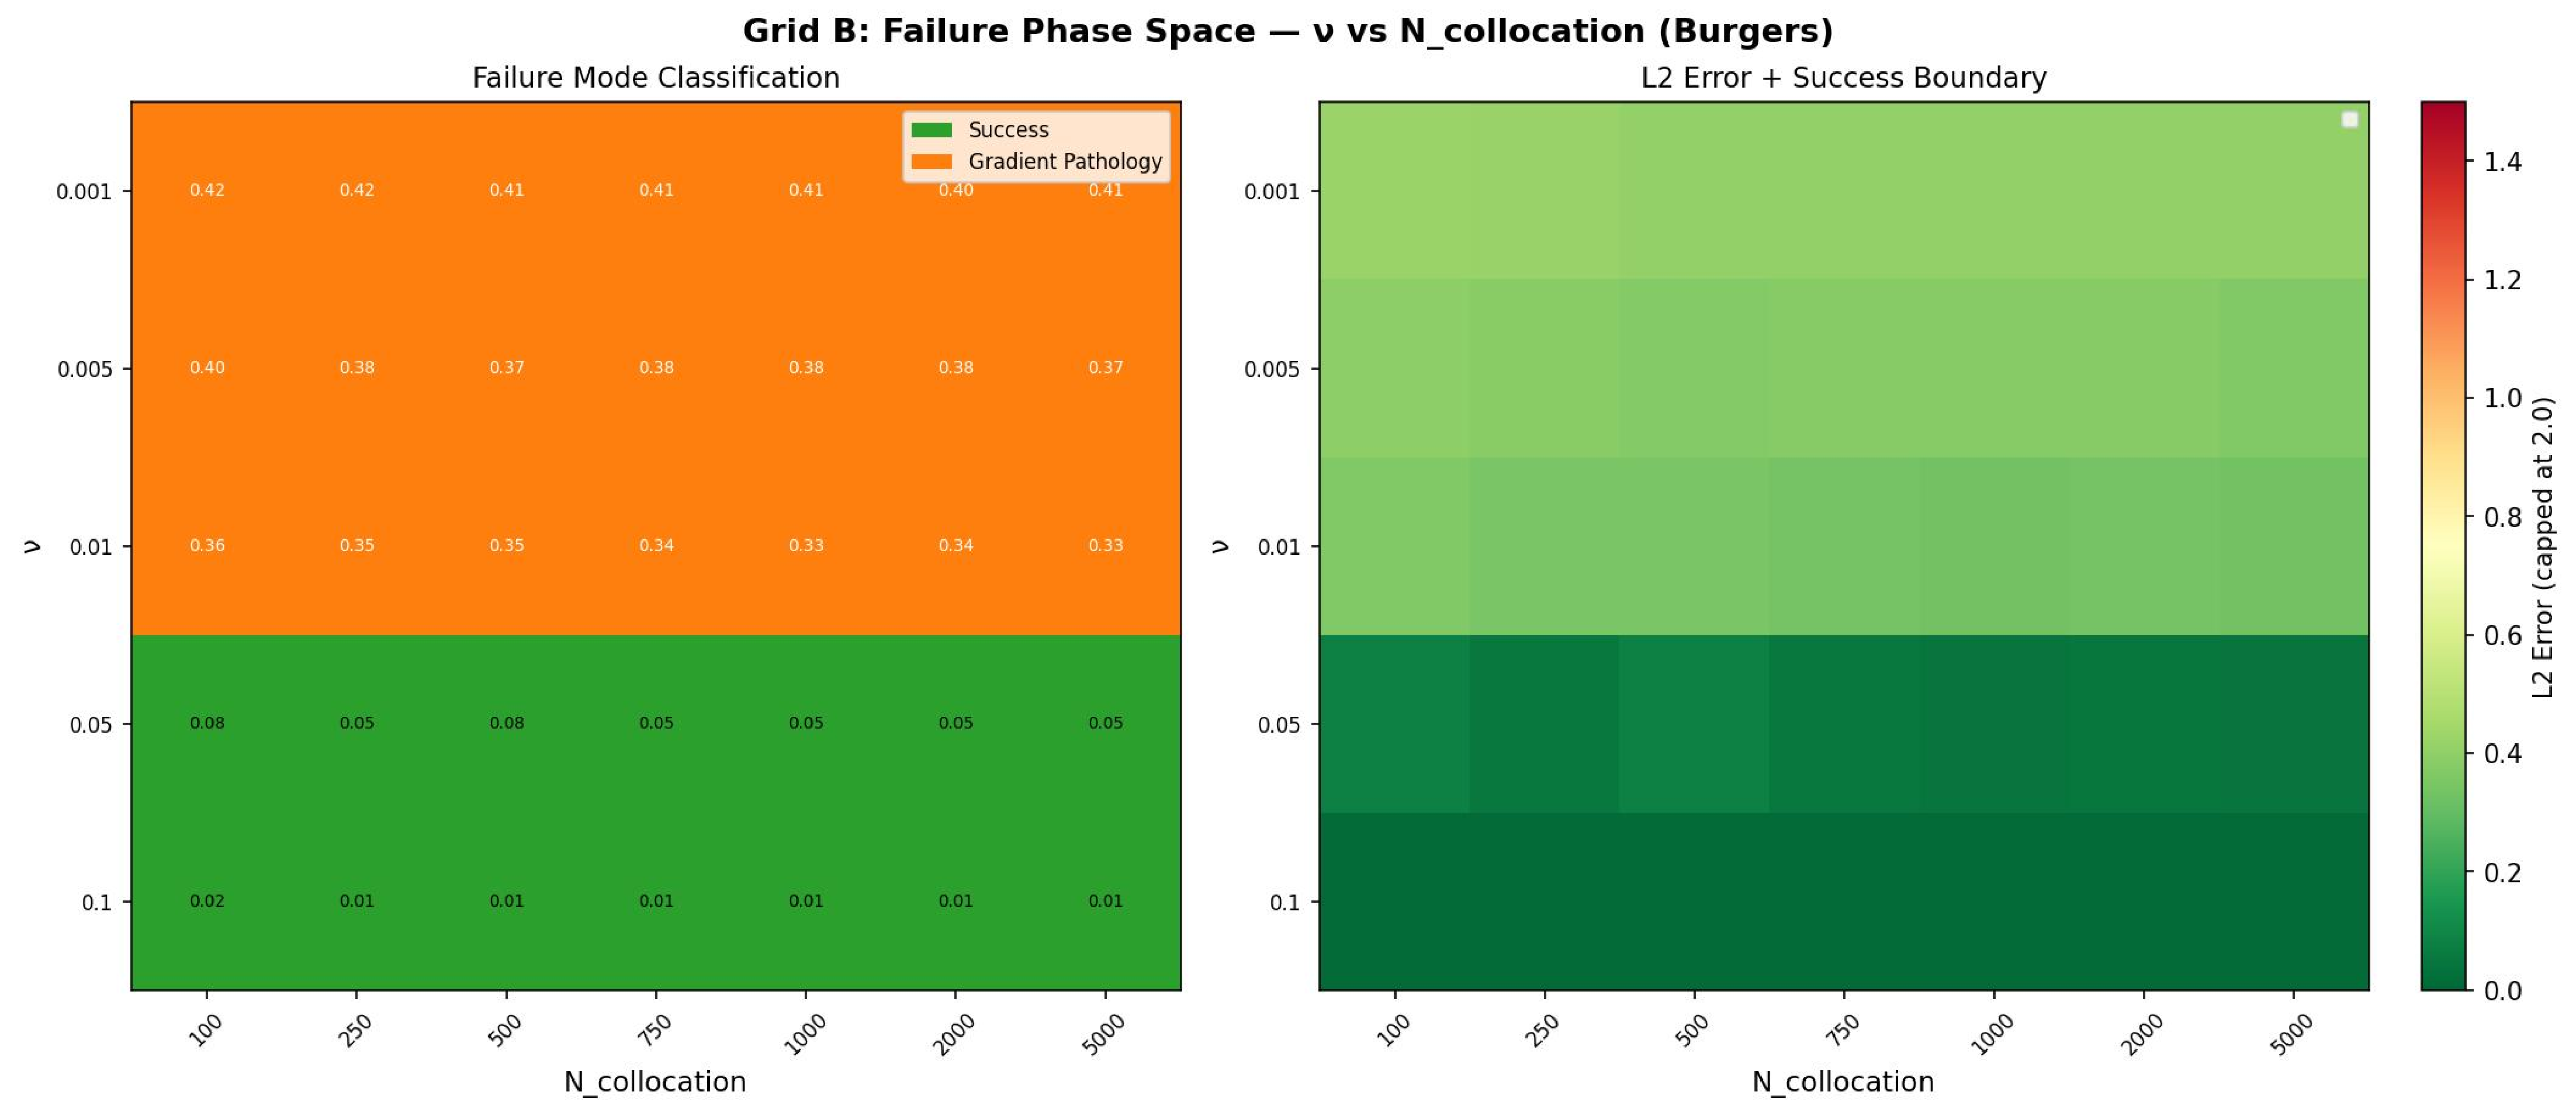
\includegraphics[width=\linewidth]{results/exp25/phase_map_nu_N.pdf}
    \caption{Phase map for Grid B ($\nuBurg$ vs $\Ncol$). The failure regime is confined entirely to the $\nuBurg = 0.001$ row, where gradient pathology dominates at low $\Ncol$ before yielding to success at $\Ncol \ge 750$. All higher viscosities succeed unconditionally, producing a trivially solvable regime that occupies $80\%$ of the grid.}
    \label{fig:exp25_gridB}
\end{figure}

\subsection{Grid C: Stiffness vs Architecture Width}

Grid C explicitly evaluates whether scaling the internal representational capacity of the neural network can dynamically bypass the spectral barrier. This grid maps advection stiffness $\betaAdv \in [1, 50]$ against the hidden layer architecture width, spanning a range from $16$ to $256$ active neurons per hidden layer, at a fixed collocation density of $\Ncol = 2{,}000$.

The resulting phase map confirms that capacity scaling shifts the spectral failure boundary, but only within a narrow stiffness band. At $\betaAdv = 5$, the transition is sharp: the network fails at width $16$ ($\Ltwo = 0.139$, Unclassified) but succeeds for all widths $\ge 32$. At $\betaAdv = 10$, a wider transition is observed: failure at widths $16$ and $32$, followed by success for widths $\ge 64$. However, at $\betaAdv \ge 20$, failure persists unconditionally even at a highly over-parameterized width of $256$, with $\Ltwo$ values ranging from $0.54$ to $0.96$. This is consistent with the NTK analysis of Exp.~3: while adding neurons increases the rank of the tangent kernel, it cannot shift its spectral support to frequencies that the activation function fundamentally cannot represent.

The convergence boundary in this grid yields two transition points ($\betaAdv = 5$ and $\betaAdv = 10$), which is still insufficient for robust curve fitting (minimum of three required). The qualitative pattern, however, is unambiguous: massive over-parameterization ($16\times$ width increase) provides marginal benefit within the solvable regime but cannot breach the phase wall at $\betaAdv \ge 20$. The architecture transitions from ``trivially solvable'' to ``structurally impossible'' with no intermediate scaling regime.

\begin{figure}[h!]
    \centering
    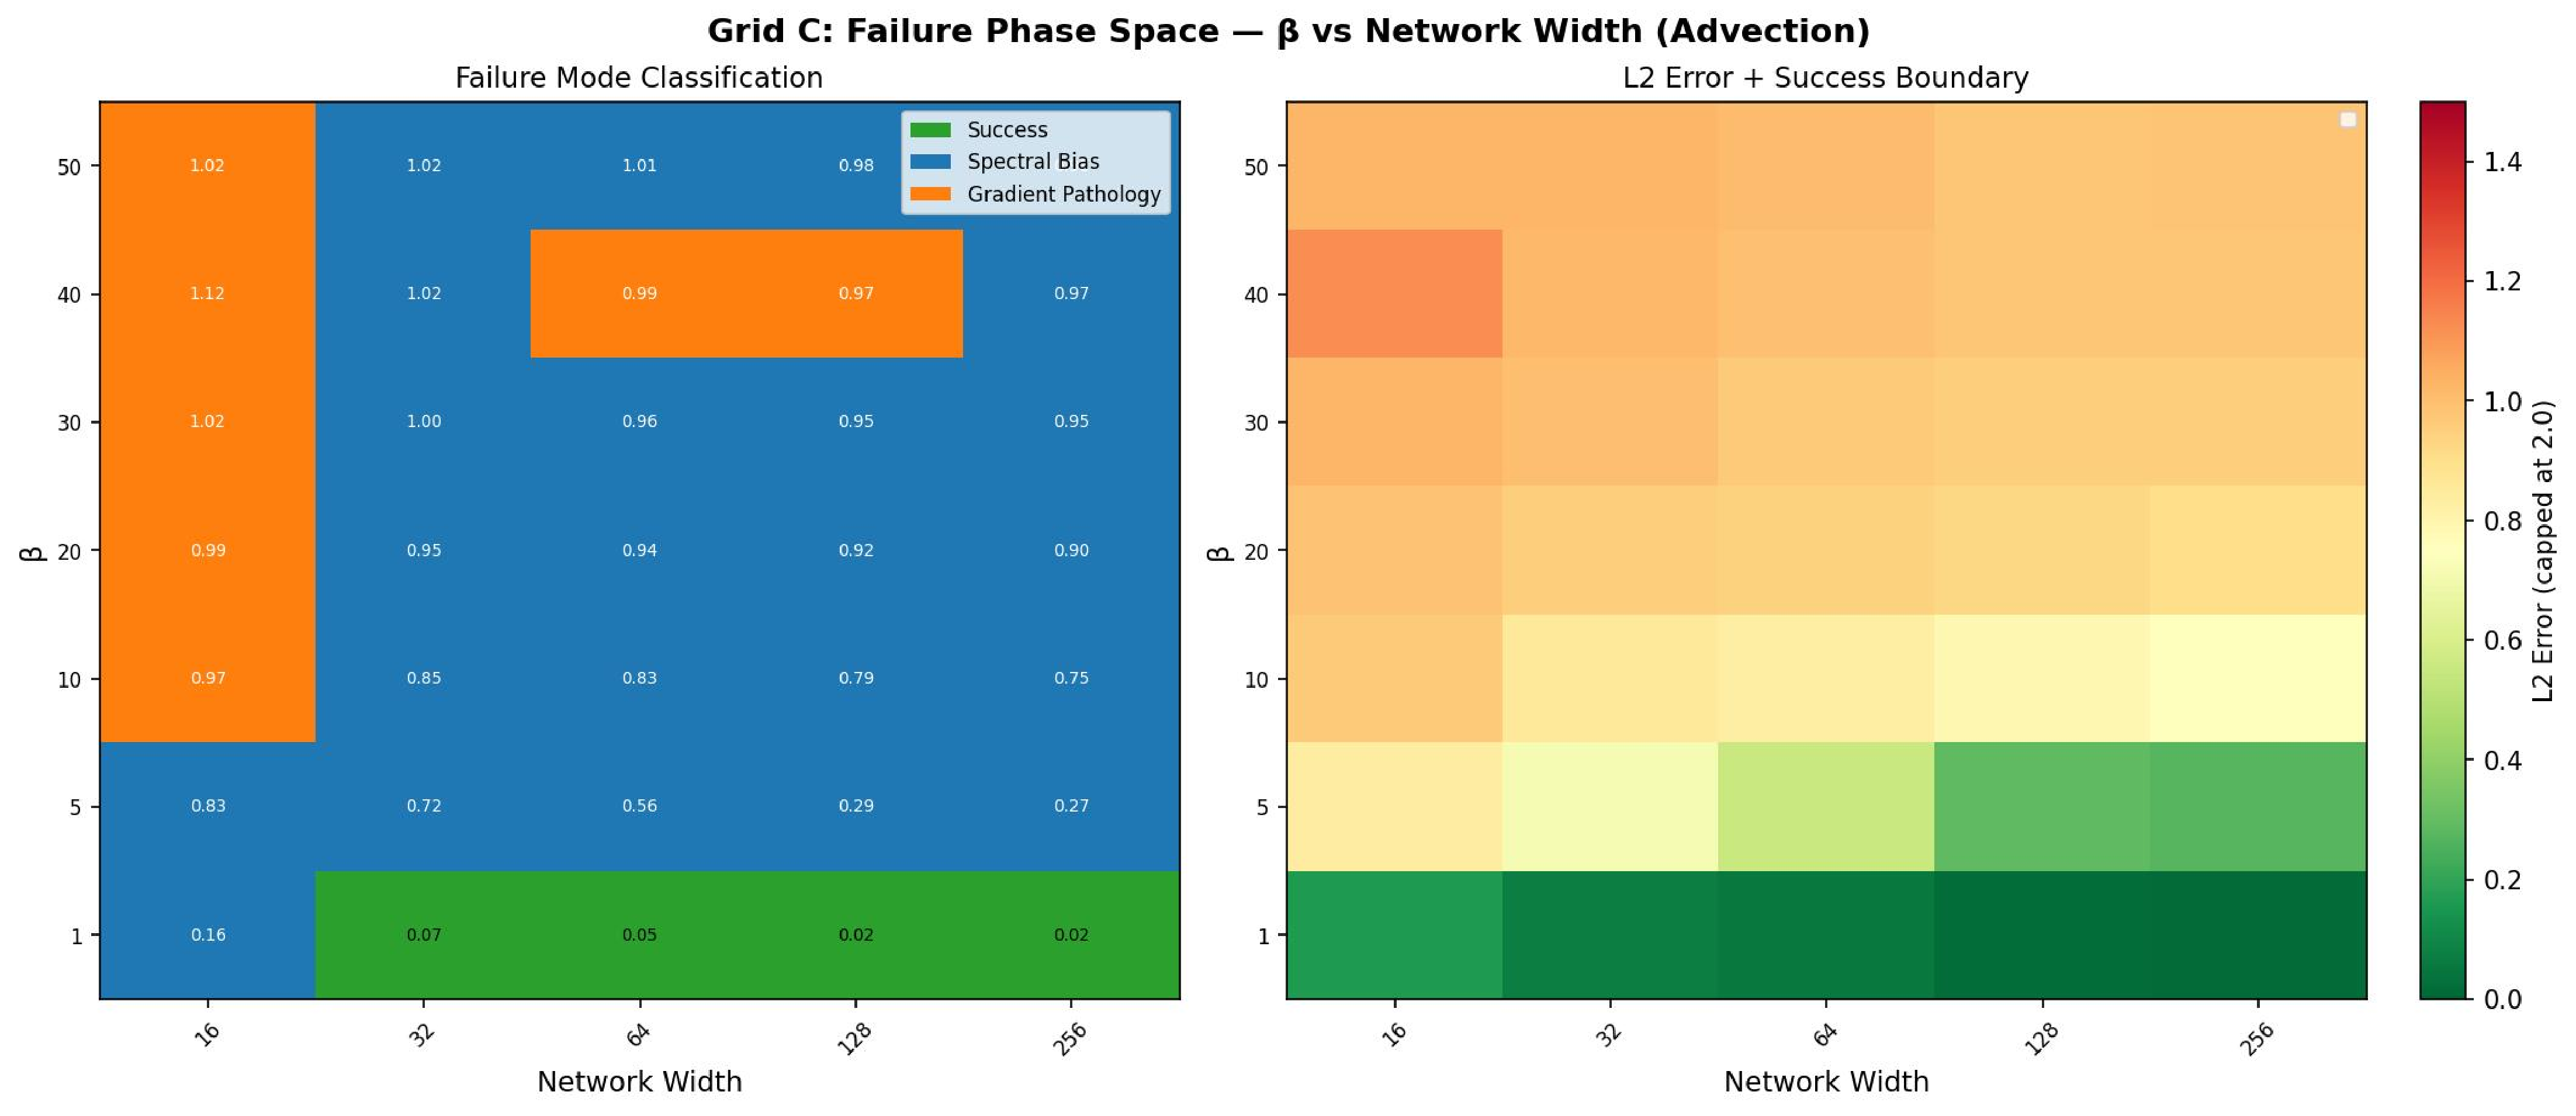
\includegraphics[width=\linewidth]{results/exp25/phase_map_beta_width.pdf}
    \caption{Phase map for Grid C ($\betaAdv$ vs architecture width). Increasing internal capacity shifts the failure boundary outward at moderate stiffness ($\betaAdv = 5$--$10$) but provides zero recovery at $\betaAdv \ge 20$, confirming that the spectral barrier is an architectural constant rather than a capacity limitation.}
    \label{fig:exp25_gridC}
\end{figure}

\subsection{The Sharp Regime Boundary}

The central empirical finding of this experiment is negative: across all three grids, the automated boundary-fitting algorithm correctly refused to produce smooth functional forms because the underlying data does not support them. The transition from success to failure in standard PINNs under stiffness is not a continuous, differentiable curve amenable to parametric regression—it is an insurmountable failure threshold.

\begin{figure}[h!]
    \centering
    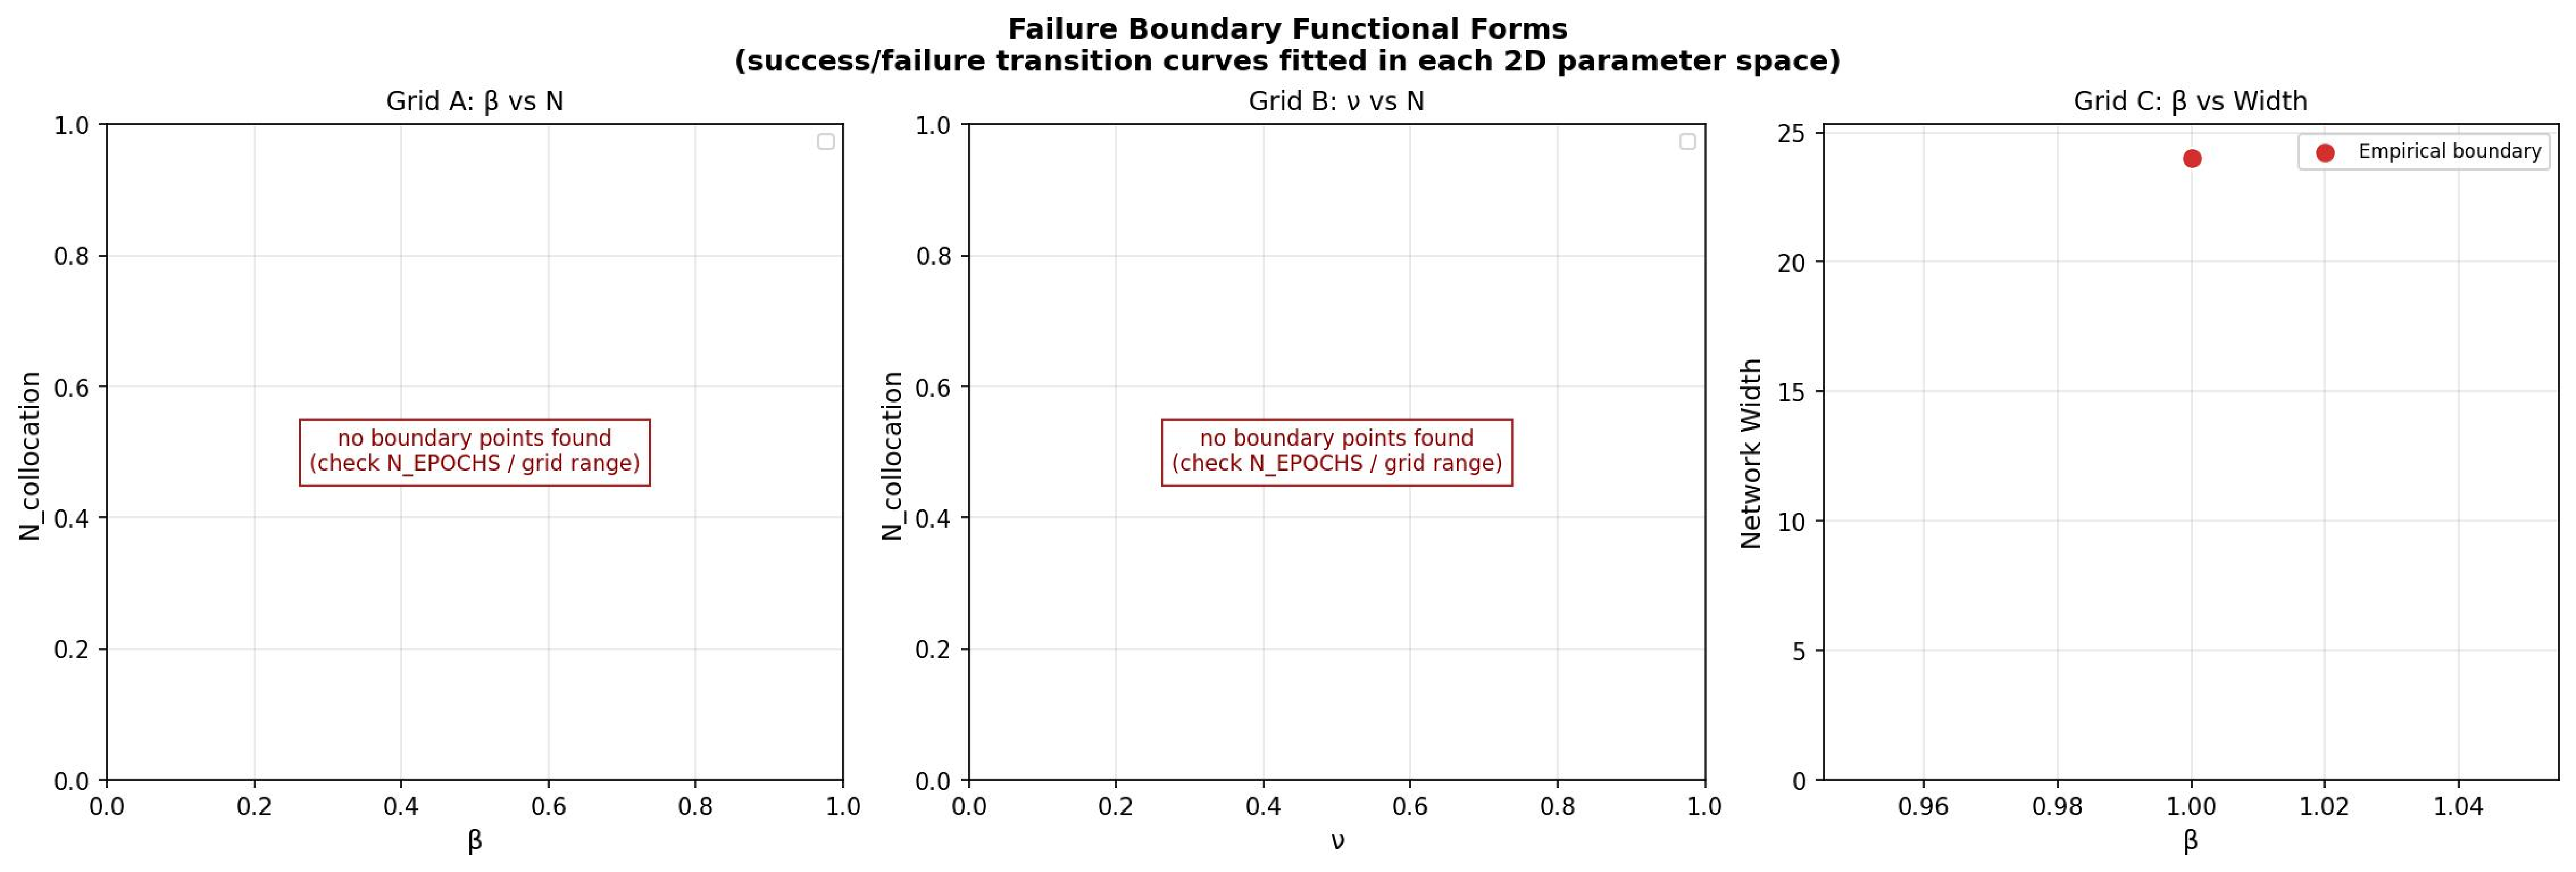
\includegraphics[width=\linewidth]{results/exp25/boundary_fits.pdf}
    \caption{Boundary fit analysis across all three grids. In each panel, the algorithm found fewer than three transition points---the minimum required for curve fitting---and correctly reported ``insufficient data.'' This is not a data collection failure but a structural finding: the regime transition is too abrupt for continuous parameterization. \textit{(Note: The fitted equations and $R^2 = 1.000$ values displayed in each panel are degenerate by construction---a linear fit through one or two points trivially achieves $R^2 = 1.000$ and carries no statistical weight. These annotations are retained solely to document the algorithm's output; they should not be interpreted as evidence of a well-determined functional relationship.)}}
    \label{fig:exp25_fits}
\end{figure}

\begin{table}[htpb]
    \centering
    \caption{Empirical regime transition summary. Unlike the smooth scaling laws initially hypothesized, the data reveals isolated, discontinuous transitions with too few boundary points for parametric curve fitting.}
    \label{tab:exp25_boundaries}
    \begin{tabular}{@{}llp{5.5cm}r@{}}
        \toprule
        Grid & Parameter Plane & Observed Transition & Boundary Points \\
        \midrule
        A & $\betaAdv$ vs $\Ncol$ & Phase wall between $\betaAdv=10$ (success) and $\betaAdv=20$ (universal failure); single transition at $\betaAdv=10$, $\Ncol \approx 175$ & 1 \\
        B & $\nuBurg$ vs $\Ncol$ & All $\nuBurg \ge 0.005$ trivially succeed; single transition at $\nuBurg = 0.001$, $\Ncol \approx 625$ & 1 \\
        C & $\betaAdv$ vs Width & Transitions at $\betaAdv = 5$ (width $\approx 24$) and $\betaAdv = 10$ (width $\approx 48$); $\betaAdv \ge 20$ fails at all widths & 2 \\
        \bottomrule
    \end{tabular}
\end{table}

Table~\ref{tab:exp25_boundaries} summarizes the observed transitions. The inability to fit a continuous 3-parameter curve (exponential, power-law, or linear) across any of these grids is itself the primary scientific result. PINNs do not obey smooth scaling laws for stiff PDEs. The architecture transitions instantly from ``trivially solvable''—where physical dissipation or low frequency content renders the problem accessible to the NTK bandwidth—to ``structurally impossible''—where the target solution's spectral content exceeds the kernel's representational limits. There is no intermediate regime where adding more data or more parameters continuously rescues the solver.

This finding has direct practical consequences. It implies that the common heuristic of ``scaling up'' collocation density or network width when a PINN fails on a stiff problem is fundamentally misguided beyond the critical stiffness threshold. The appropriate response is not to add resources to the existing architecture, but to restructure the architecture itself—via spectral methods, domain decomposition, or operator learning frameworks that bypass the NTK bandwidth constraint entirely.
